\documentclass[aspectratio=169,11pt]{beamer}
\usepackage[utf8]{inputenc}
\usepackage[T5]{fontenc}
\usepackage[vietnamese]{babel}
\usepackage{lmodern}
\usepackage{graphicx}
\usepackage{booktabs,tabularx,array}
\usepackage{tikz}
\usetikzlibrary{positioning,calc}
\usetheme{Madrid}
\usecolortheme{spruce}
\setbeamertemplate{navigation symbols}{}
\setbeamertemplate{section in toc}[sections numbered]
\setbeamercolor{section in toc}{fg=red!70!black}
\setbeamercolor{subsection in toc}{fg=blue!70!white}
\setbeamercolor{section number projected}{bg=orange,fg=white}
\graphicspath{{figures/}}

\date{Tháng 11, 2026}
\author{Nhóm Propensity VSF}
\institute{EDA dữ liệu Dunnhumby}
\title{Khám phá dữ liệu để chốt khung thời gian dự báo}
\subtitle{Từ hành vi giao dịch đến đề xuất window $T$ và horizon $H$}
\titlegraphic{\IfFileExists{fit-logo.jpg}{\includegraphics[width=3.2cm]{fit-logo.jpg}}{}}
\setbeamertemplate{title page}{%
\centering\vspace{0.5cm}\inserttitlegraphic\par\vspace{0.25cm}
\begin{beamercolorbox}[sep=8pt,center,rounded=true,shadow=true]{title}\usebeamerfont{title}\textbf{\inserttitle}\par\end{beamercolorbox}
\vspace{0.25cm}{\usebeamerfont{subtitle}\insertsubtitle\par}\vspace{0.35cm}
\begin{beamercolorbox}[sep=5pt,center]{author}\insertauthor\end{beamercolorbox}
\begin{beamercolorbox}[sep=5pt,center]{institute}\insertinstitute\end{beamercolorbox}
\vspace{0.25cm}{\small\insertdate\par}}

\newcommand{\src}[1]{\par\vfill{\tiny\color{gray}Nguồn: #1}}
\newcommand{\stat}[2]{{\Large\bfseries\color{structure.fg}#1}\quad {\small #2}\par\medskip}
\newcommand{\code}[1]{\texttt{\detokenize{#1}}}
\newcolumntype{Y}{>{\raggedright\arraybackslash}X}
\newcolumntype{C}[1]{>{\centering\arraybackslash}p{#1}}

\begin{document}

\begin{frame}[plain]\titlepage\end{frame}

\begin{frame}{Câu hỏi EDA cần trả lời}
\begin{columns}[T]
\column{.52\textwidth}
\textbf{Bài toán giữ nguyên}
\begin{itemize}
\item Tại mỗi snapshot $t$, dự báo household có mua lại trong tương lai gần hay không.
\item Feature chỉ dùng giao dịch trước hoặc tại $t$.
\item Nhãn nằm hoàn toàn sau $t$ để tránh leakage.
\end{itemize}
\medskip
\begin{block}{Hai tham số cần chốt}
$T$: số ngày lịch sử dùng để tạo feature.\\
$H$: số ngày tương lai dùng để gán nhãn mua lại.
\end{block}
\column{.44\textwidth}
\centering
\begin{tikzpicture}[x=.075\textwidth,y=1cm]
\fill[blue!18] (0,0) rectangle (7.2,1.05);
\fill[orange!32] (7.2,0) rectangle (10,1.05);
\draw[thick] (7.2,-.15)--(7.2,1.2);
\node[align=center] at (3.6,.53){\textbf{Observation window}\\lịch sử $T$ ngày};
\node[align=center] at (8.6,.53){\textbf{Target horizon}\\tương lai $H$ ngày};
\node[below,font=\scriptsize] at (0,0){$t-T+1$};
\node[below,font=\scriptsize] at (7.2,0){snapshot $t$};
\node[below,font=\scriptsize] at (10,0){$t+H$};
\end{tikzpicture}
\vspace{.55cm}
\begin{alertblock}{Phạm vi buổi này}
Chốt thiết kế thời gian ở cấp bài toán. Chưa chọn commodity và chưa kết luận về \code{CHEESE}.
\end{alertblock}
\end{columns}
\src{Thiết kế EDA của nhóm Propensity VSF.}
\end{frame}

\section{Dữ liệu có đủ nền tảng hay không}

\begin{frame}{Dữ liệu đủ dài và đủ lặp lại để làm propensity theo thời gian}
\begin{columns}[T]
\column{.46\textwidth}
\stat{2.595.732}{product lines}
\stat{276.484}{baskets}
\stat{2.500}{households}
\stat{711 ngày}{tương đương 102 tuần}
\column{.50\textwidth}
\textbf{Grain và độ phủ đã được xác nhận}
\begin{itemize}
\item Một dòng là một sản phẩm trong một basket.
\item Cặp \code{BASKET_ID + PRODUCT_ID} không trùng.
\item DAY liên tục từ 1 đến 711, chưa gắn ngày lịch thực.
\item Median household có 79 baskets, 70 active days và span 627 ngày.
\item 2.461/2.500 household có span ít nhất 365 ngày.
\end{itemize}
\medskip
\alert{Hệ quả:} có thể tạo nhiều snapshot lịch sử và kiểm tra quyết định $T$, thay vì chọn từ một cutoff cuối.
\end{columns}
\src{transaction\_data.csv; notebook 01 và 04.}
\end{frame}

\begin{frame}{Population gần như đã hình thành từ đầu observation window}
\centering
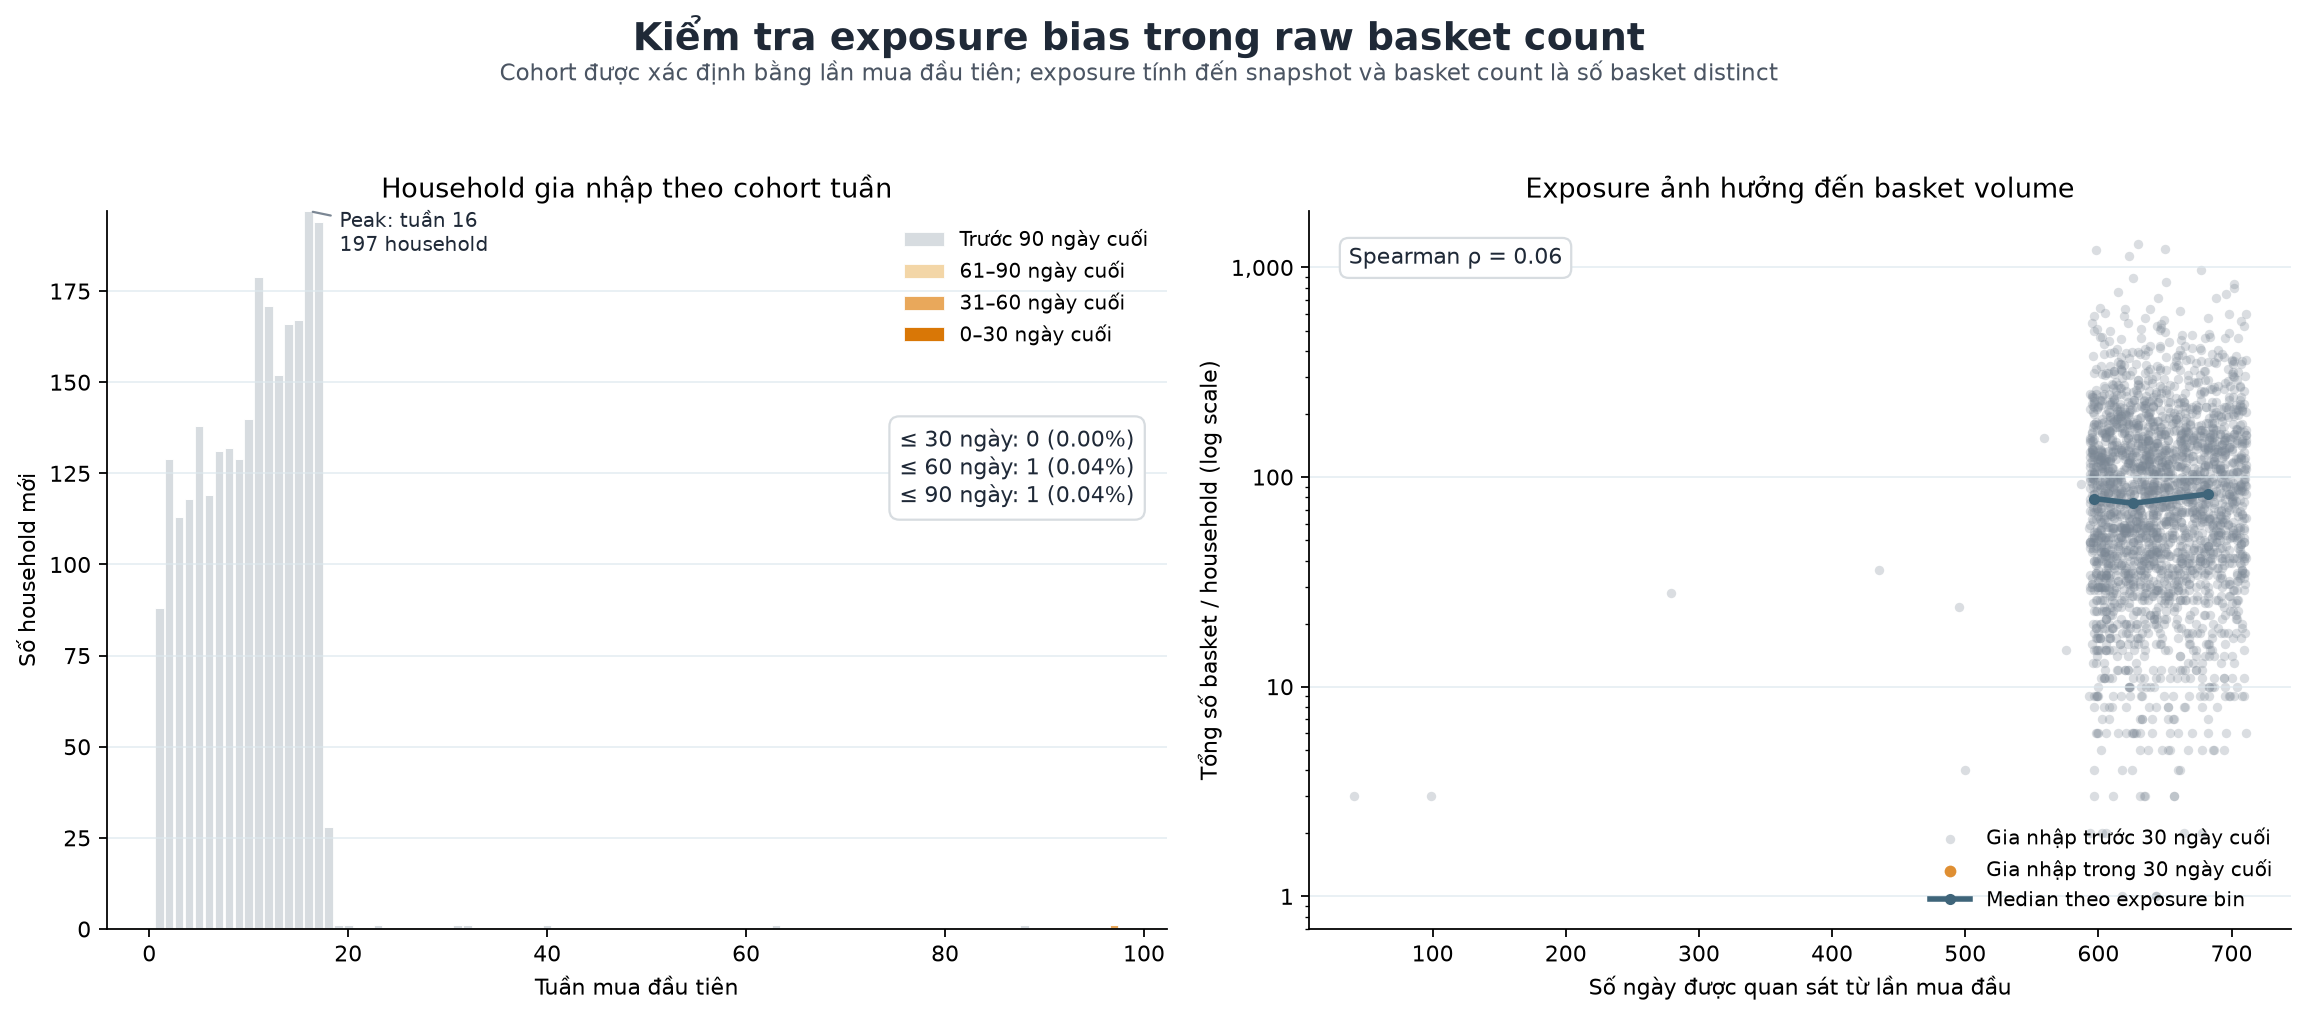
\includegraphics[width=.91\textwidth]{lifecycle_coverage_exposure.png}
\vspace{-.15cm}
\begin{columns}[T]
\column{.47\textwidth}\small
Chỉ 1 household gia nhập trong 60--90 ngày cuối và không có household nào gia nhập trong 30 ngày cuối.
\column{.47\textwidth}\small
Spearman giữa exposure và basket count chỉ bằng 0,06. Raw frequency hiện không bị exposure chi phối mạnh.
\end{columns}
\src{Notebook 04, 2.500 households tại DAY 711.}
\end{frame}

\section{Household mua lại theo nhịp nào}

\begin{frame}{Đa số household vẫn hoạt động gần snapshot}
\centering
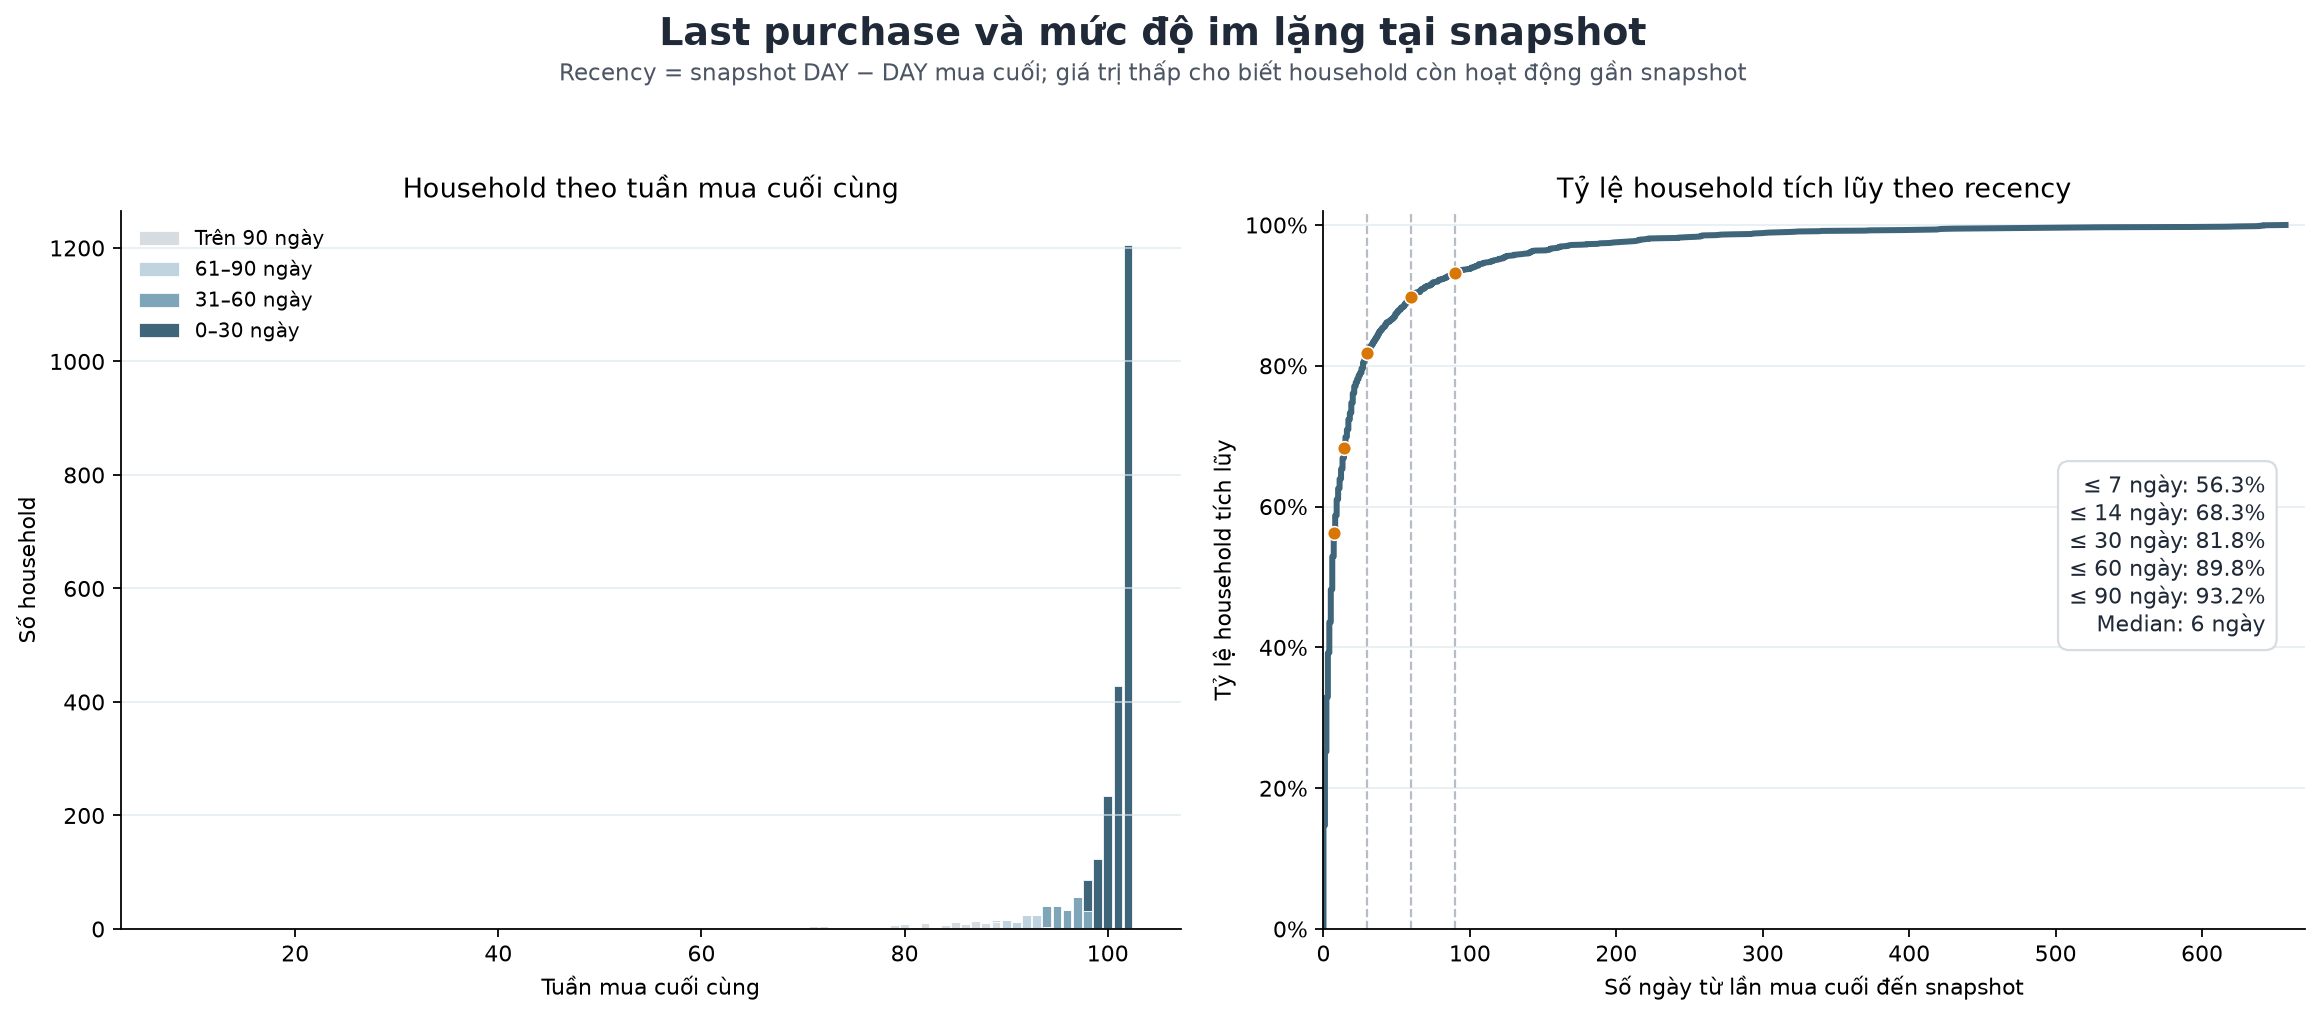
\includegraphics[width=.91\textwidth]{last_purchase_recency.png}
\vspace{-.15cm}
\begin{columns}[T]
\column{.30\textwidth}\centering
\textbf{6 ngày}\\[-1mm]\small median recency
\column{.30\textwidth}\centering
\textbf{68,3\%}\\[-1mm]\small mua trong 14 ngày
\column{.30\textwidth}\centering
\textbf{93,2\%}\\[-1mm]\small mua trong 90 ngày
\end{columns}
\src{Notebook 04, recency tại snapshot DAY 711.}
\end{frame}

\begin{frame}{Khoảng quay lại tập trung mạnh trong hai tuần}
\centering
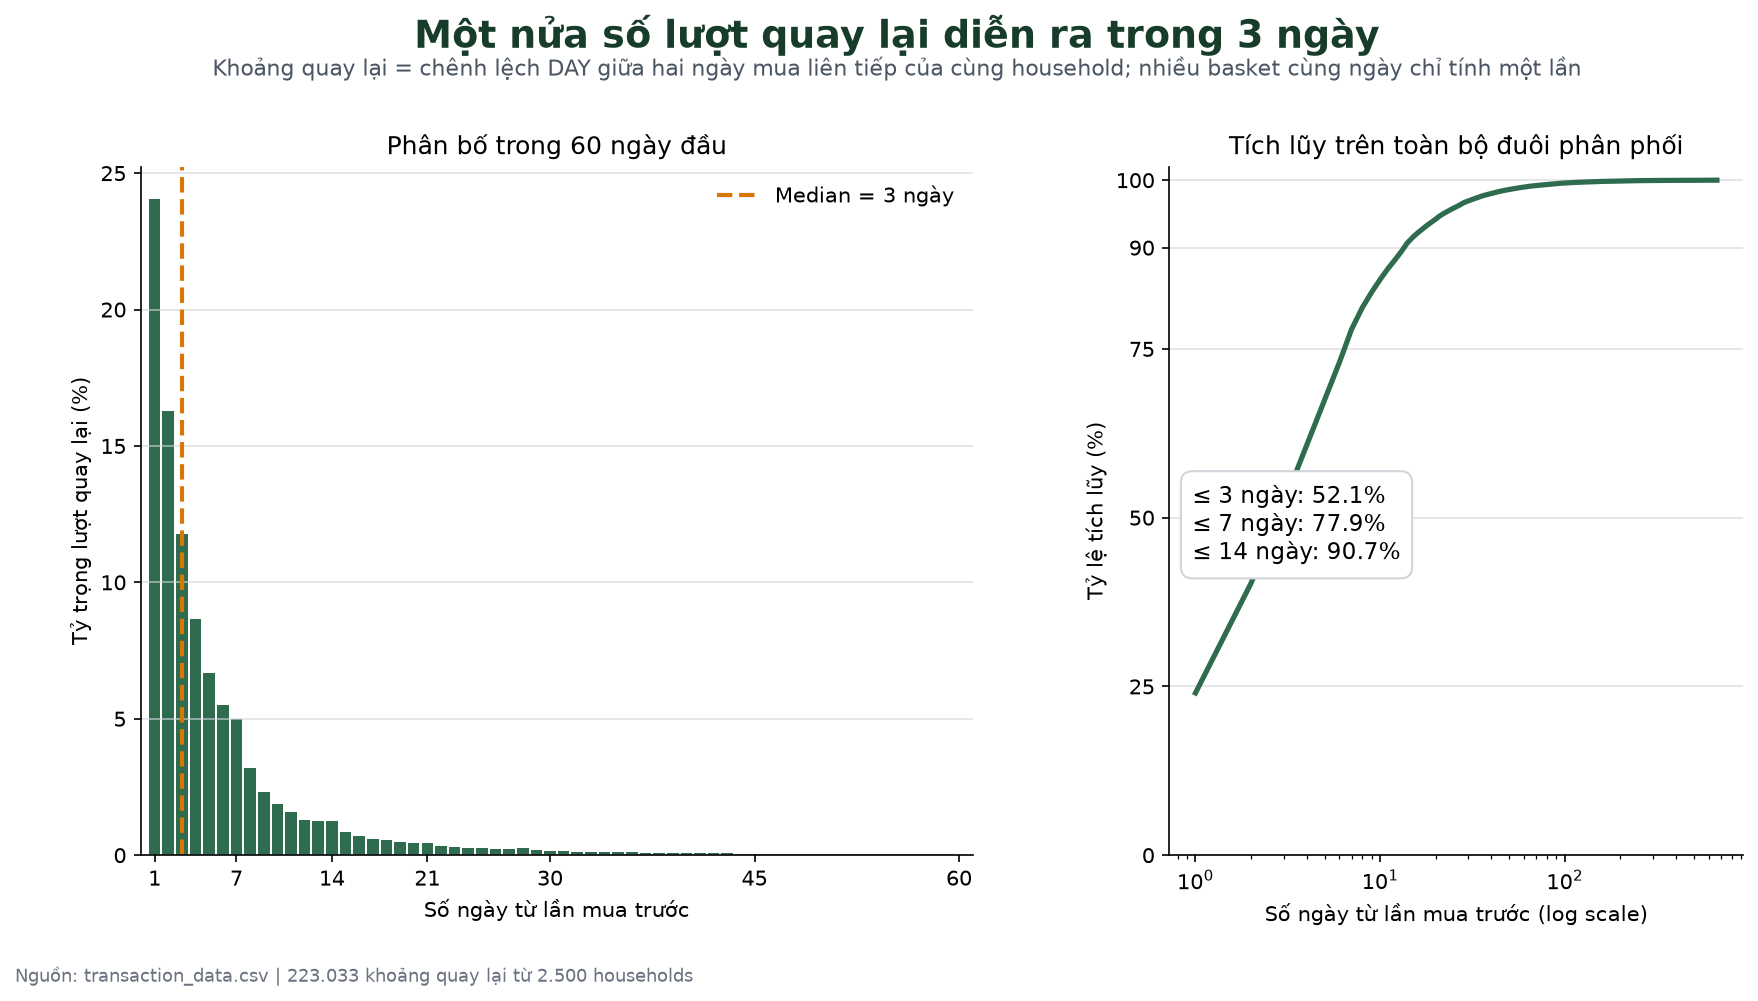
\includegraphics[width=.91\textwidth]{return_interval_distribution.png}
\vspace{-.05cm}
\begin{columns}[T]
\column{.47\textwidth}\small
223.033 khoảng quay lại hợp lệ. Median event-level là 3 ngày, p90 là 14 ngày và p95 là 22 ngày.
\column{.47\textwidth}\small
90,7\% lượt quay lại xảy ra trong 14 ngày. Sau mốc này, phần tăng thêm của target coverage giảm rõ.
\end{columns}
\src{transaction\_data.csv; khoảng cách giữa hai active days liên tiếp.}
\end{frame}

\begin{frame}{Nhịp mua nhanh nhưng không đều giữa các household}
\begin{columns}[T]
\column{.49\textwidth}
\textbf{Population-level}
\begin{itemize}
\item Median lượt quay lại là 3 ngày.
\item 77,9\% quay lại trong 7 ngày.
\item 90,7\% quay lại trong 14 ngày.
\end{itemize}
\column{.47\textwidth}
\textbf{Household-level}
\begin{itemize}
\item Median của chu kỳ trung vị theo household là 6 ngày.
\item Mật độ CV chính nằm quanh 0,7--1,3.
\item 30,1\% household đang trễ hơn hai lần nhịp mua riêng tại snapshot.
\end{itemize}
\end{columns}
\medskip
\begin{alertblock}{Ý nghĩa cho thiết kế nhãn}
$H$ phải đủ dài để bắt phần lớn lượt mua lại, nhưng không nên kéo dài đến mức gộp nhiều chu kỳ và làm nhãn bão hòa. Mốc 14 ngày cân bằng hai yêu cầu này ở EDA toàn danh mục.
\end{alertblock}
\src{Notebook 04, 223.033 intervals và 2.479 household đủ regularity evidence.}
\end{frame}

\section{Bao nhiêu lịch sử là đủ}

\begin{frame}{Window ngắn đo recency tốt nhưng thiếu bằng chứng về cadence}
\centering
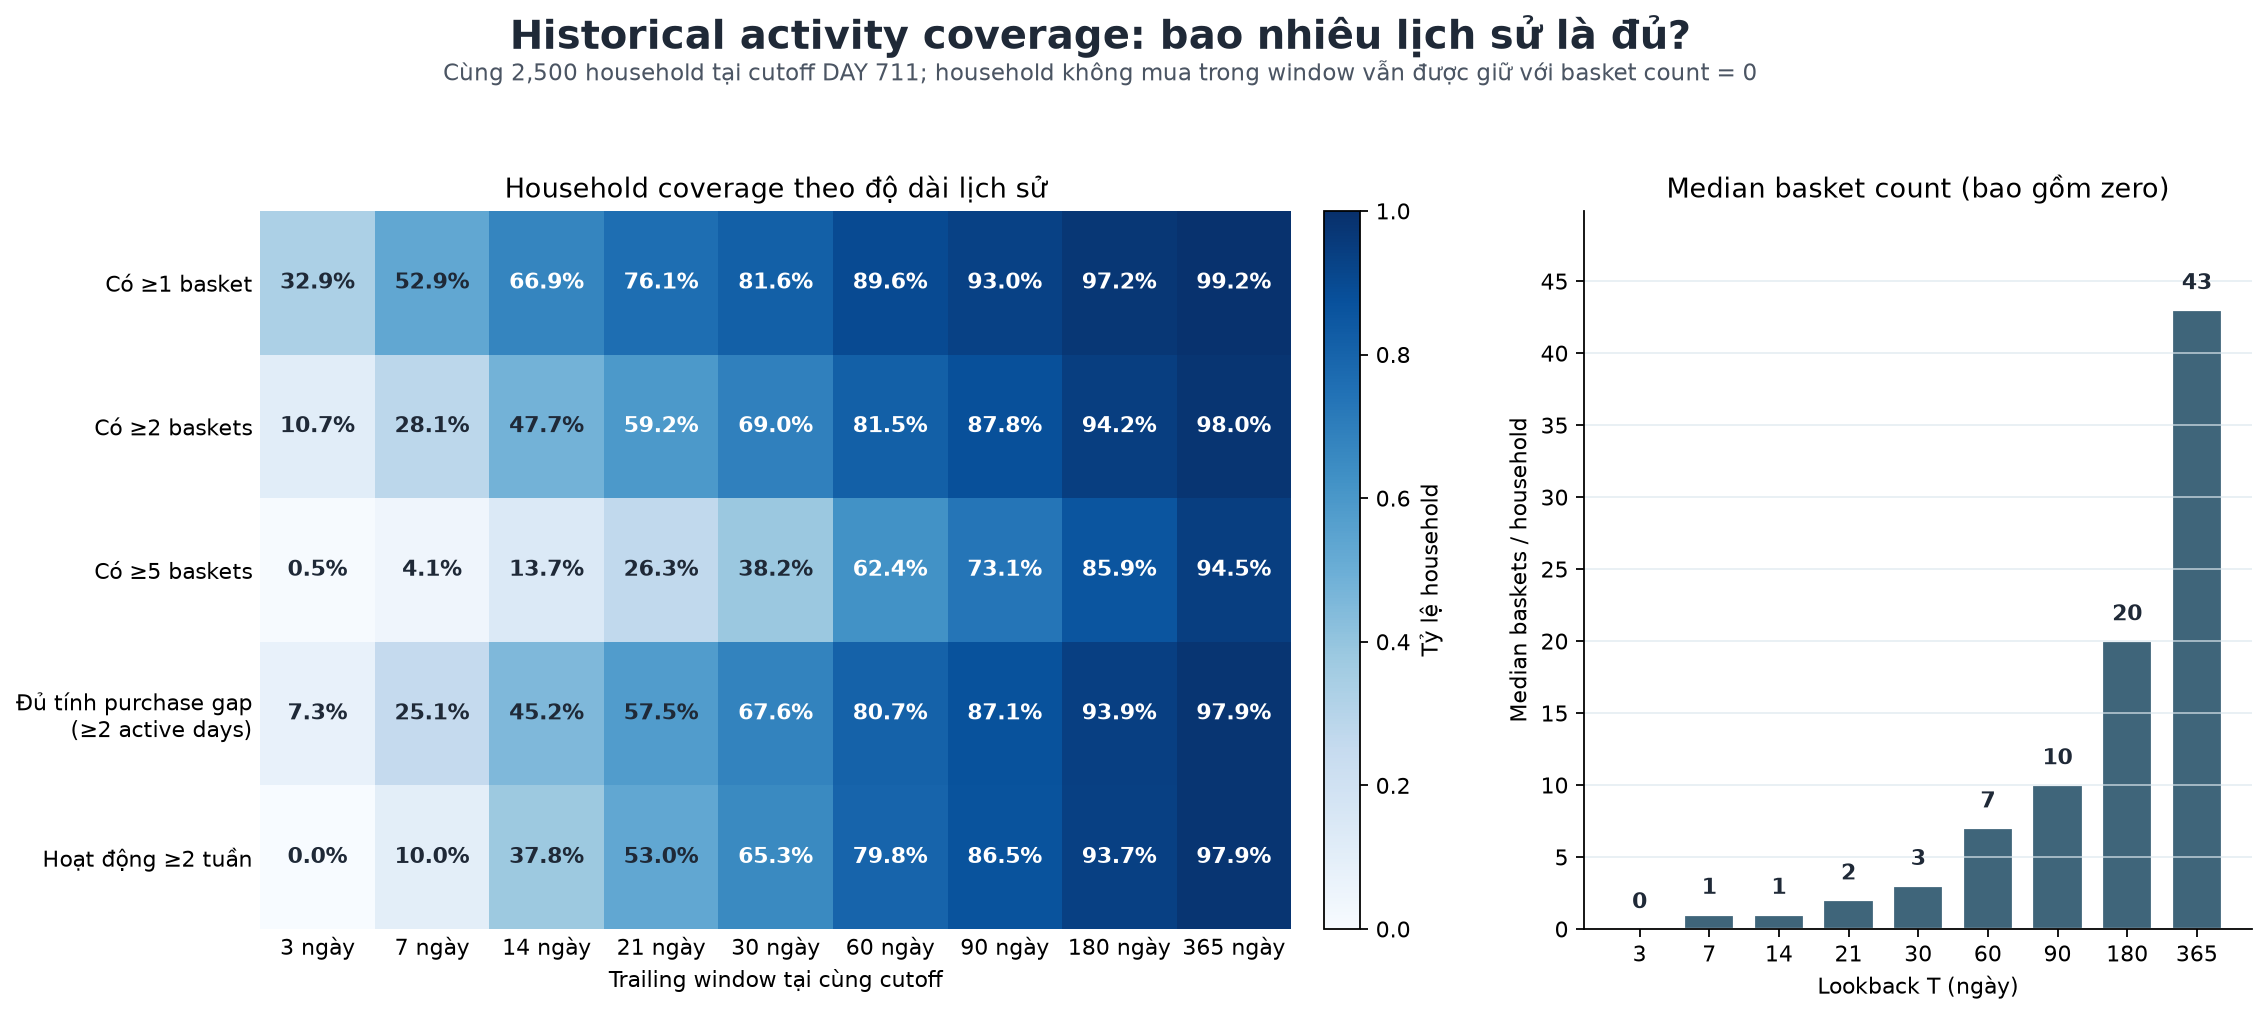
\includegraphics[width=.91\textwidth]{historical_activity_coverage.png}
\vspace{-.12cm}
\begin{columns}[T]
\column{.30\textwidth}\small
\textbf{$T=30$ ngày}\\
67,6\% gap-ready, median 3 baskets.
\column{.30\textwidth}\small
\textbf{$T=90$ ngày}\\
87,1\% gap-ready, median 10 baskets.
\column{.30\textwidth}\small
\textbf{$T=180$ ngày}\\
93,9\% gap-ready, 85,9\% có ít nhất 5 baskets.
\end{columns}
\src{Notebook 04, cùng 2.500 household tại cutoff DAY 711; zero activity vẫn được giữ.}
\end{frame}

\begin{frame}{Kết luận về $T$ ổn định qua nhiều historical cutoffs}
\centering
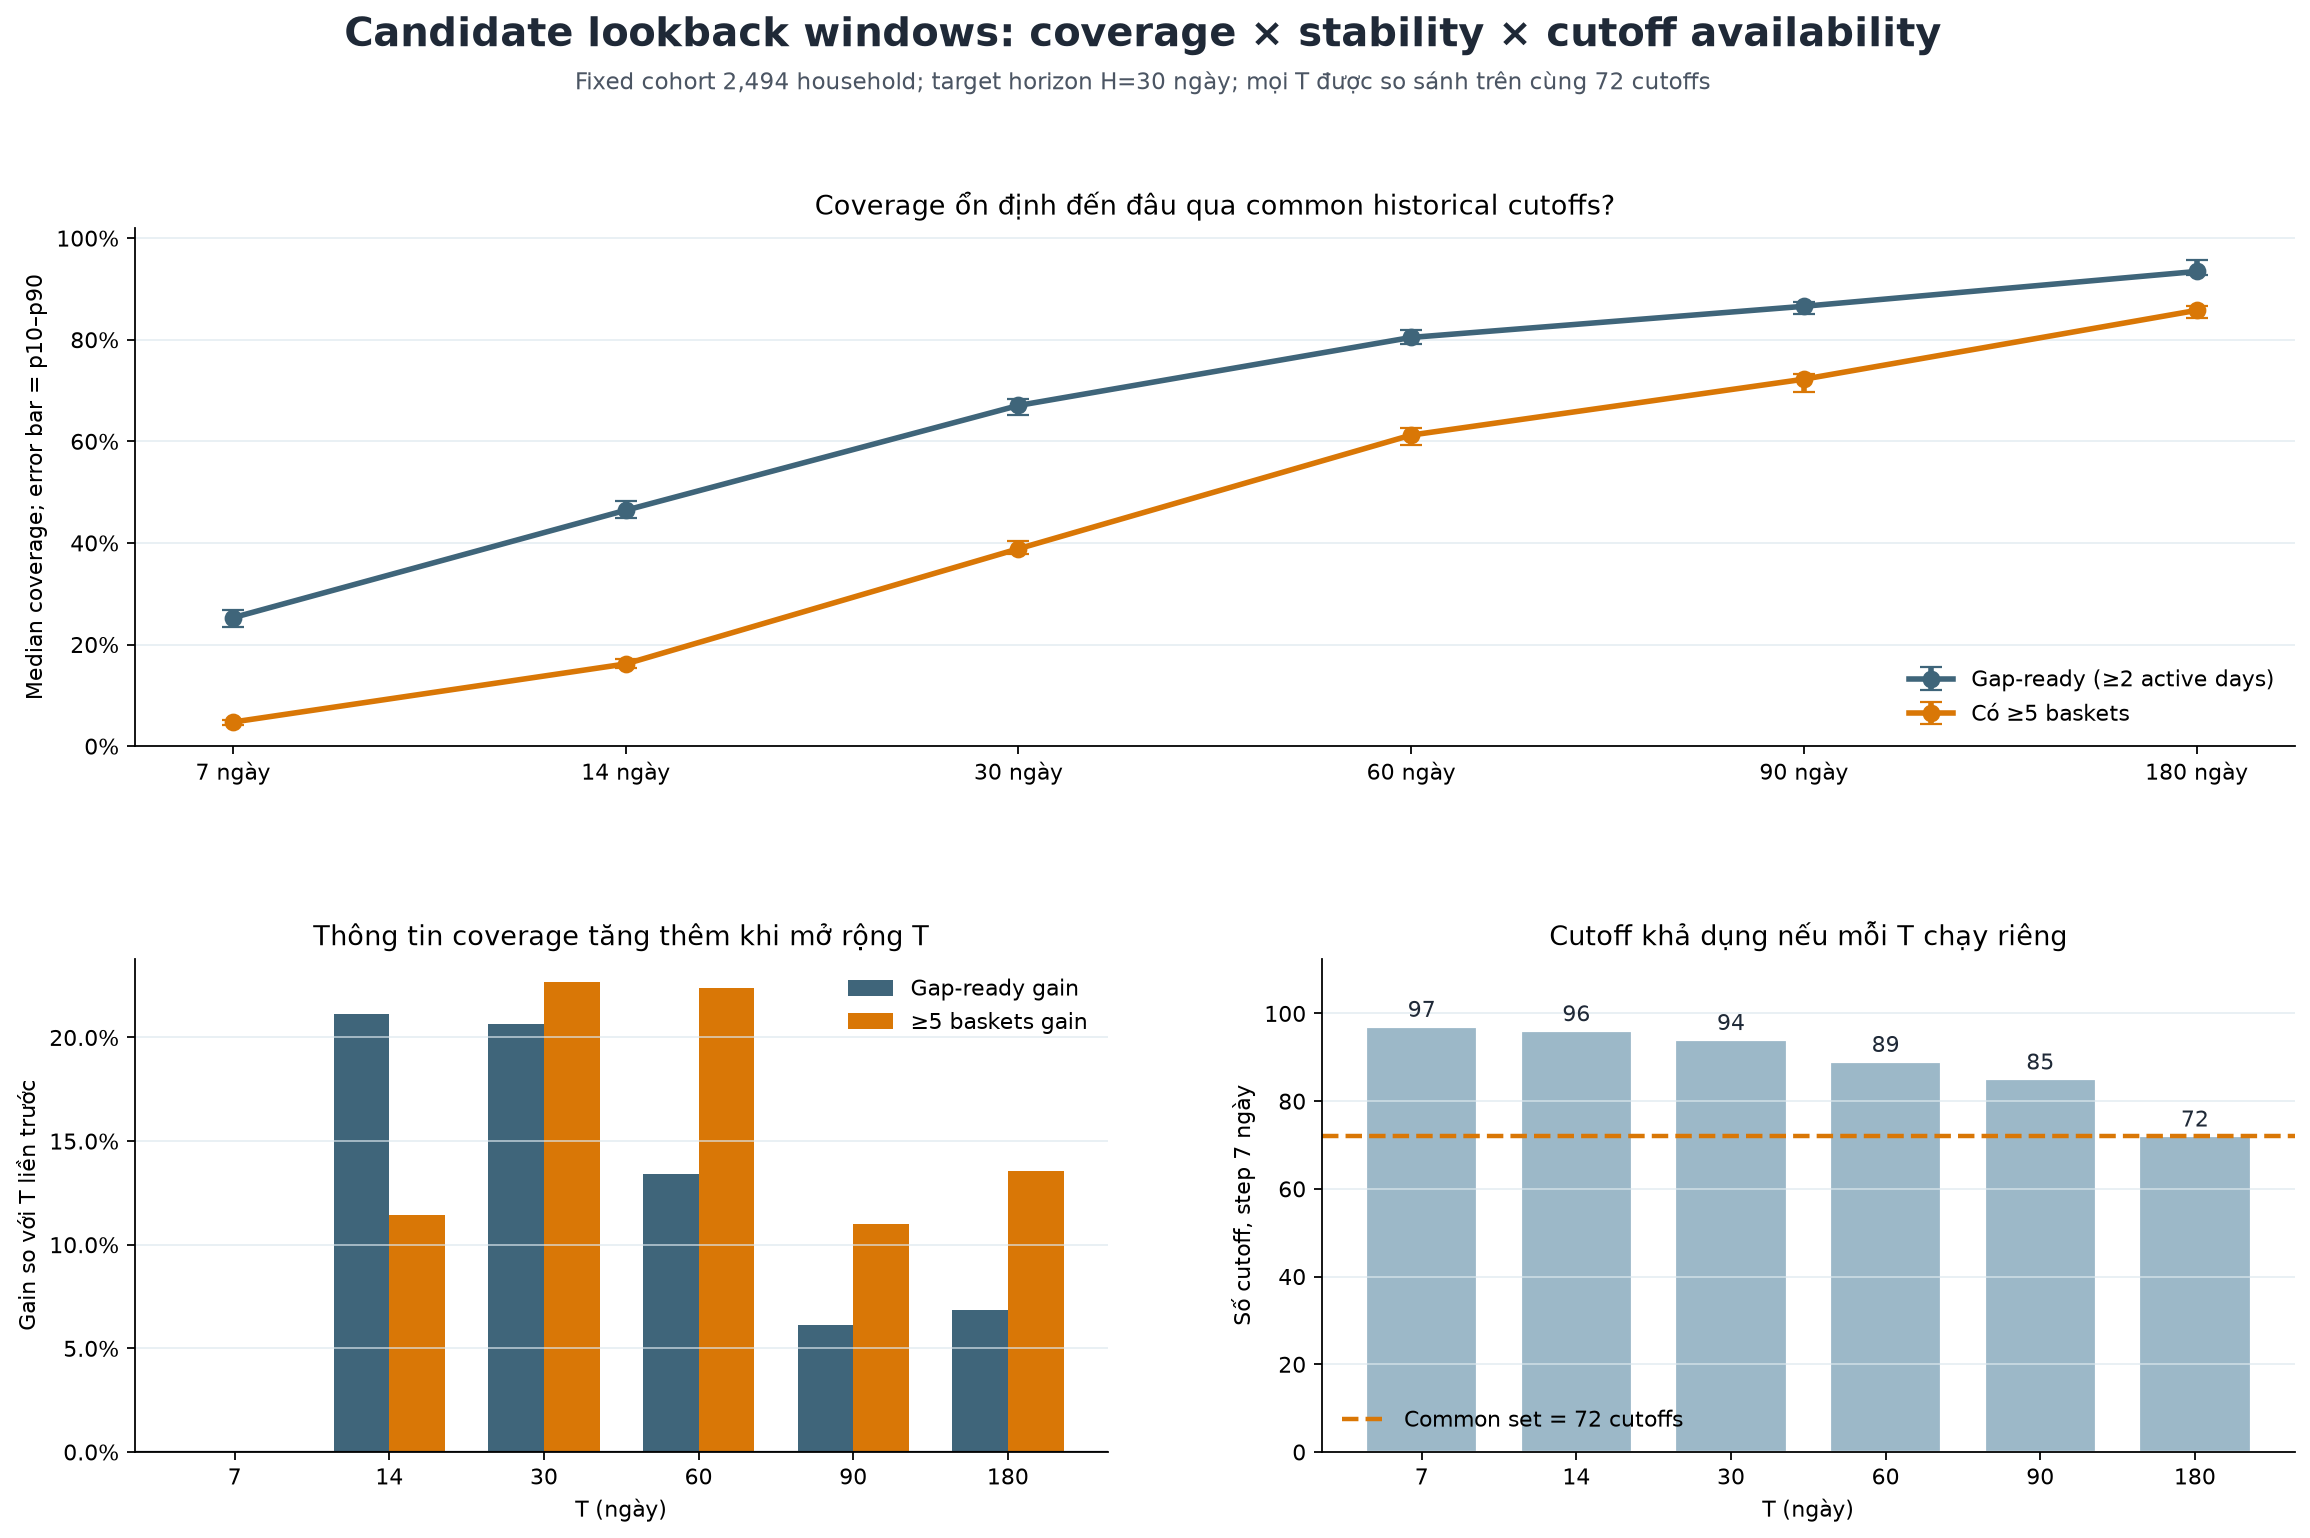
\includegraphics[width=.89\textwidth]{window_candidate_evidence.png}
\vspace{-.12cm}
\begin{columns}[T]
\column{.46\textwidth}\small
Trên 72 common cutoffs, $T=90$ đạt median 86,6\% gap-ready và 72,2\% household có ít nhất 5 baskets.
\column{.46\textwidth}\small
Biểu đồ dùng $H=30$ như stress test về cutoff availability. Các coverage metrics của $T$ chỉ dùng lịch sử trước snapshot.
\end{columns}
\src{Notebook 04; candidates 7/14/30/60/90/180 ngày, cutoff cách nhau 7 ngày.}
\end{frame}

\begin{frame}{Một window duy nhất bỏ sót thay đổi hành vi gần đây}
\centering
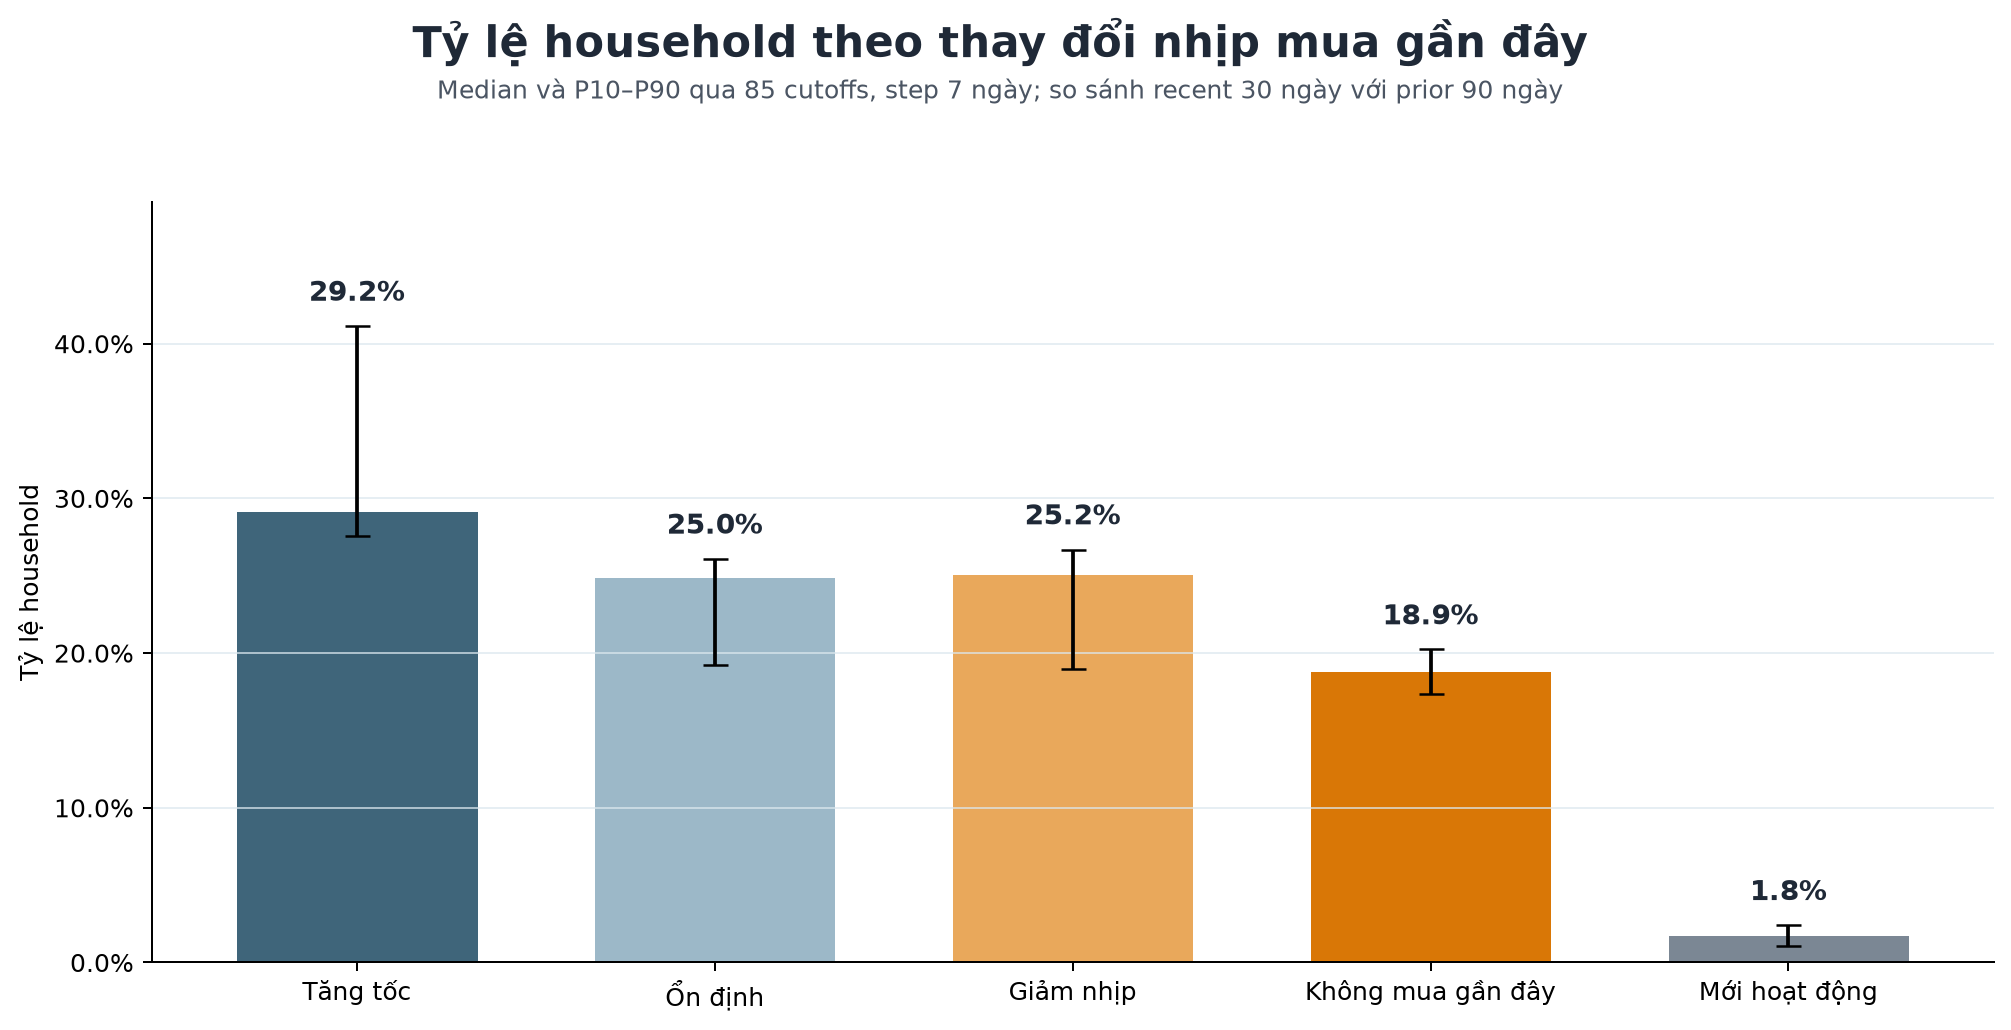
\includegraphics[width=.88\textwidth]{household_behavior_shift.png}
\vspace{-.15cm}
\begin{columns}[T]
\column{.30\textwidth}\small
Median 29,2\% household tăng tốc qua 85 cutoffs.
\column{.30\textwidth}\small
25,2\% giảm nhịp và 18,9\% không mua gần đây.
\column{.30\textwidth}\small
Nhóm giảm nhịp tăng median basket size từ 5 lên 7.
\end{columns}
\src{Notebook 04; recent 30 vs prior 90 ngày, 85 cutoffs cách 7 ngày, fixed cohort.}
\end{frame}

\section{Đề xuất thiết kế thời gian}

\begin{frame}{Đề xuất kiểm chứng: $H=7$, bắt đầu với $T=30$}
\begin{columns}[T]
\column{.52\textwidth}
\centering
\resizebox{\linewidth}{!}{%
\begin{tikzpicture}[x=1cm,y=1cm]
\fill[green!22] (0,0) rectangle (7.5,1.15);
\fill[orange!35] (7.5,0) rectangle (10,1.15);
\draw[thick] (7.5,-.18)--(7.5,1.3);
\node[align=center] at (3.75,.58){\Large\textbf{$T=30$ ngày}\\\small hành vi gần đây};
\node[align=center] at (8.75,.58){\Large\textbf{$H=7$ ngày}\\\small nhãn mua lại};
\node[below,font=\scriptsize] at (0,0){$t-29$};
\node[below,font=\scriptsize] at (7.5,0){snapshot $t$};
\node[below,font=\scriptsize] at (10,0){$t+7$};
\end{tikzpicture}%
}
\vspace{.45cm}
\begin{block}{Cách kiểm chứng $T$}
\small
Giữ nguyên household, cutoff và cohort. Tạo cùng feature với
$T=30/60/90/180$, sau đó đo giá trị tăng thêm của lịch sử dài hơn.
\end{block}
\column{.44\textwidth}
\small
\textbf{Vì sao thử $H=7$}
\begin{itemize}\setlength\itemsep{2pt}
\item Phù hợp nhịp kích hoạt marketing hàng tuần.
\item CHEESE đạt positive rate 24,9\% trong prior buyers active 90 ngày.
\item Giữ $H=14$ làm sensitivity case; positive rate tăng lên 41,0\%.
\end{itemize}
\textbf{Vì sao bắt đầu từ $T=30$}
\begin{itemize}\setlength\itemsep{2pt}
\item Ưu tiên recency và thay đổi hành vi gần snapshot.
\item Toàn bộ giao dịch có 67,6\% household gap-ready.
\item Riêng CHEESE chỉ đạt 24,5\%; cadence cần thêm $T=90/180$.
\end{itemize}
\end{columns}
\src{Notebook 04--06; cùng cutoff và cohort khi so sánh các candidate $T/H$.}
\end{frame}

\section{CHEESE là ứng viên đầu tiên}

\begin{frame}{CHEESE đủ điều kiện để đưa vào predictive validation}
\small
\begin{tabularx}{\textwidth}{@{}p{2.6cm}p{3.0cm}Y@{}}
\toprule
\textbf{Bằng chứng} & \textbf{Kết quả CHEESE} & \textbf{Ý nghĩa cho bài toán} \\
\midrule
Quy mô & 2.350 buyers; 2.220 repeat buyers & Cohort đủ lớn để tạo household-cutoff samples \\
\addlinespace
Target tại $H=14$ & 41,0\% trong prior buyers active 90 ngày & Nhãn không quá hiếm trong scoring cohort dự kiến \\
\addlinespace
Cadence & Median gap 13 ngày; 55,6\% intervals trong 14 ngày & $H=14$ gần nhịp mua điển hình, nhưng không bao phủ toàn bộ repeat cycle \\
\addlinespace
Promotion context & 83,9\% purchase days có promotion & Commodity phù hợp với use case marketing; chưa chứng minh causal lift \\
\bottomrule
\end{tabularx}
\medskip
\begin{alertblock}{Cách diễn giải}
Các con số đủ để chọn CHEESE làm commodity thử nghiệm đầu tiên. EDA chưa chứng minh CHEESE tối ưu hơn mọi commodity.
\end{alertblock}
\src{Notebook 05; target rate là median qua common cutoffs.}
\end{frame}

\begin{frame}{Nhịp mua CHEESE ủng hộ $H=14$ nhưng coverage chỉ đạt 55,6\%}
\centering
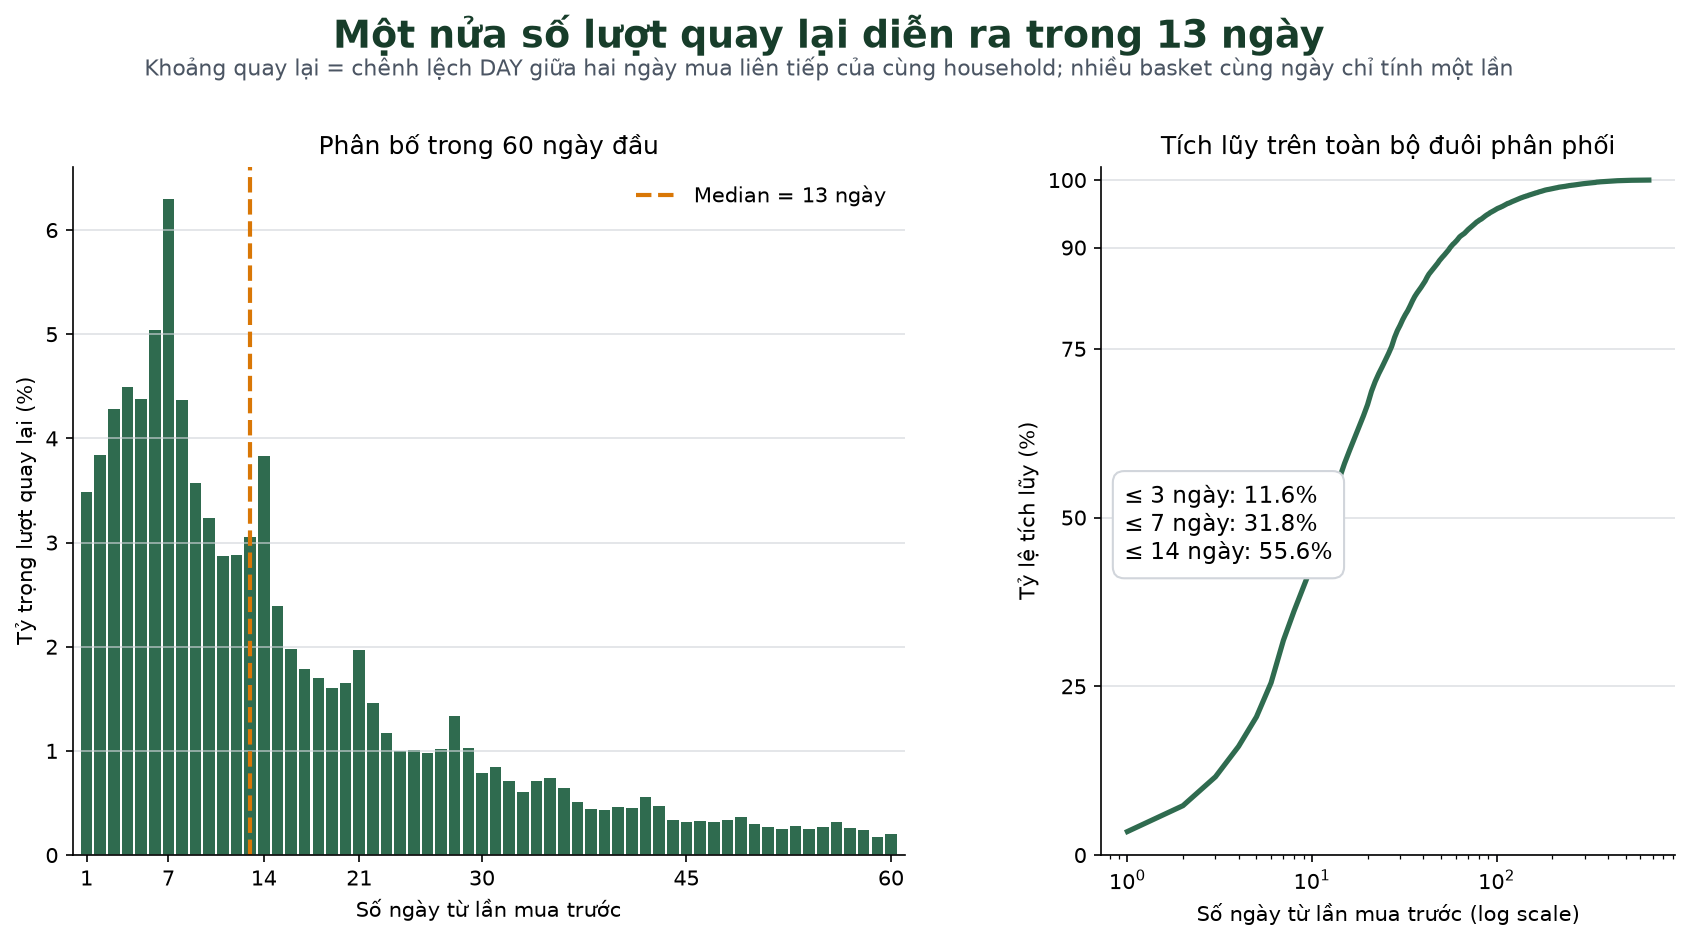
\includegraphics[width=.88\textwidth]{cheese_return_interval_distribution.png}
\vspace{-.12cm}
\begin{columns}[T]
\column{.30\textwidth}\small
\textbf{13 ngày}\\
Median khoảng mua lại CHEESE.
\column{.30\textwidth}\small
\textbf{55,6\%}\\
Intervals nằm trong 14 ngày.
\column{.30\textwidth}\small
\textbf{41,0\%}\\
Positive rate trong active-90d buyers.
\end{columns}
\src{Notebook 05 và 06; 43.767 repeat intervals của CHEESE.}
\end{frame}

\begin{frame}{$T=90$ còn thưa nếu feature cần cadence ổn định}
\centering
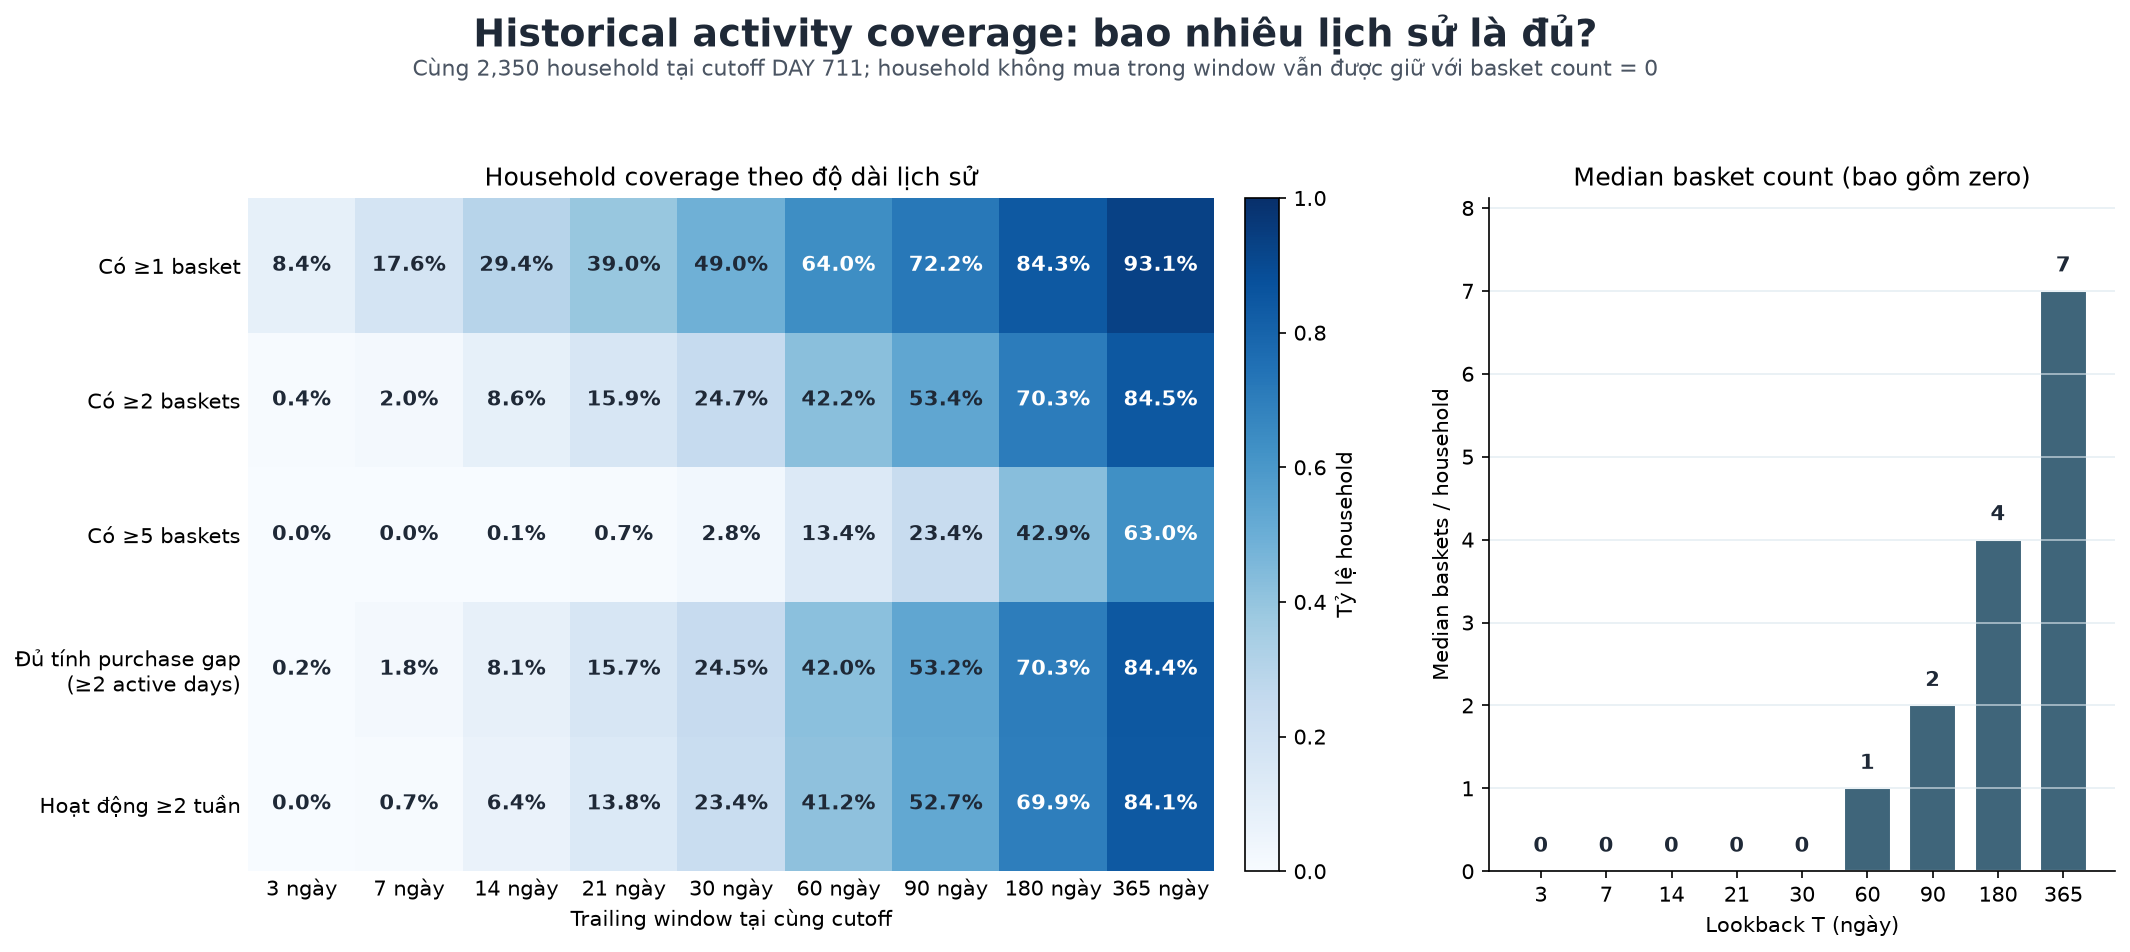
\includegraphics[width=.88\textwidth]{cheese_historical_activity_coverage.png}
\vspace{-.14cm}
\begin{columns}[T]
\column{.30\textwidth}\small
\textbf{72,2\%} có ít nhất một CHEESE basket trong 90 ngày.
\column{.30\textwidth}\small
\textbf{53,2\%} đủ hai active days để tính purchase gap.
\column{.30\textwidth}\small
Chỉ \textbf{23,4\%} có ít nhất 5 baskets; median bằng 2.
\end{columns}
\medskip
\centering\small
$T=90$ phù hợp cho recency, frequency và eligibility. Regularity, CV và trend cần thêm $T=180$.
\src{Notebook 06; 2.350 CHEESE buyers tại cutoff DAY 711.}
\end{frame}

\begin{frame}{Đề xuất để xin ý kiến}
\begin{columns}[T]
\column{.48\textwidth}
\textbf{Phương án nhóm đang nghiêng về}
\begin{itemize}
\item Chọn CHEESE làm commodity thử nghiệm đầu tiên.
\item Giữ $H=14$ để khớp campaign cadence và median purchase gap.
\item Dùng $T=90$ cho recency, frequency và scoring eligibility.
\item Dùng thêm $T=180$ cho cadence và regularity.
\end{itemize}
\column{.48\textwidth}
\textbf{Hai phương án thay thế}
\begin{enumerate}
\item Dùng $T=180$ cho toàn bộ feature để tăng evidence, đổi lại phản ứng chậm hơn với hành vi mới.
\item Giữ duy nhất $T=90$ nhưng giới hạn cohort ở household có ít nhất hai CHEESE purchase days.
\end{enumerate}
\end{columns}
\medskip
\begin{alertblock}{Nguyên tắc}
Xin ý kiến: nhóm có đồng ý thử CHEESE với thiết kế multi-window 30/90/180 ngày và nhãn $H=14$ hay muốn ưu tiên một window duy nhất?
\end{alertblock}
\src{Đề xuất thảo luận từ notebook 05 và 06; chưa phải cấu hình modeling cuối cùng.}
\end{frame}

\begin{frame}{Bước xác nhận trước khi modeling}
\small
\begin{tabularx}{\textwidth}{@{}p{2.6cm}Y Y@{}}
\toprule
\textbf{Kiểm tra} & \textbf{Thiết kế} & \textbf{Tiêu chí quyết định} \\
\midrule
Backtest $T$ & So sánh 30/60/90/180 ngày trên cùng cutoff và cohort & AUC/PR-AUC, calibration và độ ổn định theo cutoff \\
\addlinespace
Backtest $H$ & So sánh 7/14/21/30 ngày sau khi chọn commodity & Positive rate đủ học, phù hợp campaign cadence và có lead time hành động \\
\addlinespace
Leakage audit & Đóng băng feature tại DAY $\leq t$, nhãn ở DAY $t+1$ đến $t+H$ & Không có biến dùng thông tin sau snapshot \\
\addlinespace
Cohort policy & So sánh toàn household với prior buyers active trong $T$ & Cohort phải khớp đối tượng business có thể tác động \\
\bottomrule
\end{tabularx}
\medskip
\centering
\color{structure.fg}\bfseries Kết luận hiện tại: thử CHEESE với $H=14$; xin ý kiến về multi-window $T=30/90/180$.
\src{Đề xuất quy trình kiểm định của nhóm Propensity VSF.}
\end{frame}

\end{document}
